\chapter{PROBLEM}

The basic problem in this thesis is how to find appropriate job descriptions by user's r\'esum\'e. If we take the r\'esum\'e as a query and the job descriptions as documents, we need to build an information retrieval model to get the most relevance documents.  The JobFinder will parse the job descriptions to the job models, and store them in the database. When a user searches the jobs by their r\'esum\'e in the system, the system will compare the similarity values between the r\'esum\'e and the job models, and return the jobs sorted by their similarity values.

The core idea of our algorithm is calculate similarity between the r\'esum\'e model and job model.
We give a formal definition of our problem. All of the notations will be used frequently throughout the thesis.

We use $r$ to denote the user's r\'esum\'e model, which has some features $r_i$ like their academic degree, their major, their skills and so on. The symbol $J$ is the set of job models stored in the database, and $j$ is a job model in the set $J$. The similarity function $sim(r, j)$ gives the similarity values between r\'esum\'e $r$ and job $j$. The return list of search function $search(r,J)$ will calculate all the similarity value in the database, and the result of the function will be the job description list ranked by their similarity values. The equation of how to calculate similarity value is given below:

$$ sim(r, j) = \sum_{i=1}^{n} simfun_i(r_i,j_i) \times w_i $$

The value of $sim(r, j)$ is the summation of the similarity values of different fields times their corresponding weights. Different fields like major and skills,  may have different functions to calculate their similarity values. We will describe the similarity functions of individual fields in later parts.

\chapter{System Overview}

\section{System Overview}
The system will use rule based information extraction technique to parse job descriptions and r\'esum\'es, and get information such as skill, specialties and background. These information will be used to create the model of job openings and job seekers. Ontology will be used to construct the knowledge base, which will include the taxonomy, to support r\'esum\'e-job matching.

The models of r\'esum\'e will include job seekers' specialties, working experience and education background, all the fields will be extracted from their r\'esum\'es. The job models will be extracted from job descriptions, and have the same information fields as the r\'esum\'e models.  When a job seeker searches the jobs by his r\'esum\'e, the system will calculate the similarity between the candidate model and the job models, give every job model a similarity score.

\section{System Architecture}

Figure ~\ref{fig:Pipeline} shows the architecture of the whole system, which include such modules:

\begin{enumerate}
    \item The web scrawler could search and download all new IT job opening web pages  from indeed.com everyday.
    \item Job parser could parse the job opening web page, extract the information and create the job model.
    \item Resume Parser is much like the Job parser, it will parse the r\'esum\'e and create the candidate model.
    \item All the job models will be stored in the Job Description database.
    \item When user make a query request, the ontology matcher will calculate the matching score of each job, return the jobs ranked by their scores.
\end{enumerate}

\begin{figure}[htbp]
  \centering
  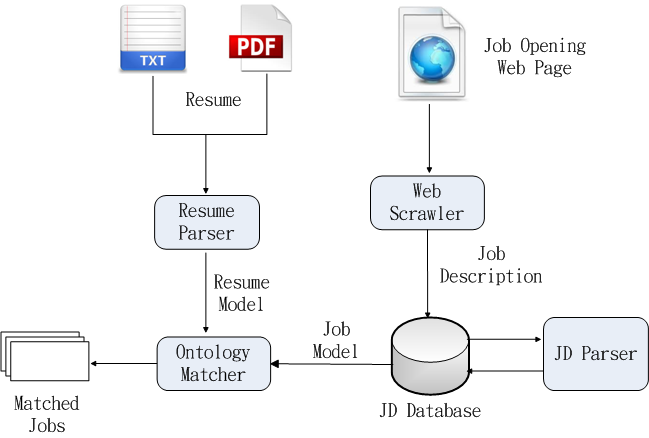
\includegraphics[scale=0.5]{images/arch.png}
  \caption{System Architecture}
  \label{fig:arch}
\end{figure}

\section{System Implementation}

We describe some implementation details here. The whole system was implemented in Python, and used some third party libraries and frameworks. For the web module we used Flask, a lightweight web framework. We used Rdflib as the OWL file parser, PLY(Python Lex-Yacc) as the token regular expression compiler, whoosh as the unversed index builder and Beautiful Soup as the HTML parser.  All the jobs get by the web crawler are stored in the MongoDB NoSQL database.  For the natural language processing part, we used NLTK and pattern to extract the sentences and tokenized the sentences.

\section{System Interface}

The system provide some interfaces to end users. The most important interfaces include the web pages reviewing all the jobs in the database, searching the jobs by keyword Figure~\ref{fig:joblist},  uploading user's r\'esum\'e ~\ref{fig:upload_resume},  matching the jobs with r\'esum\'e~\ref{fig:match_resume} and searching the jobs with both keyword and r\'esum\'e~\ref{fig:keyword_resume}.

\begin{figure}[htbp]
  \centering
  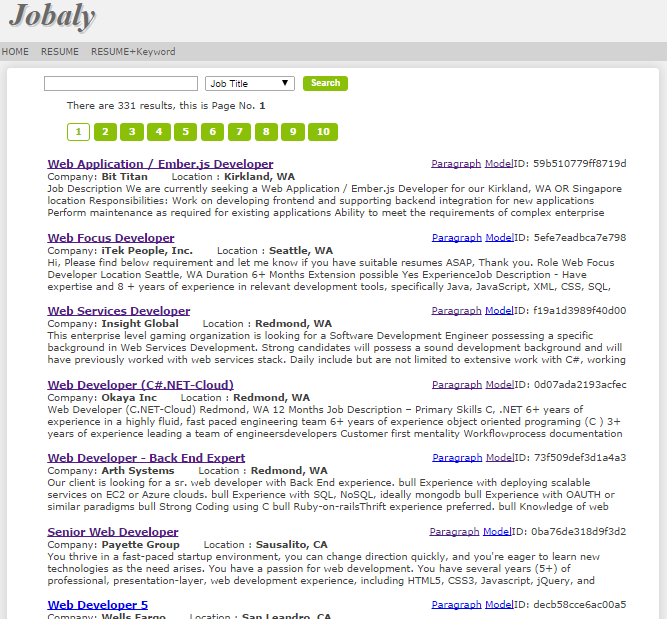
\includegraphics[scale=0.5]{images/joblist.png}
  \caption{Job Description List}
  \label{fig:joblist}
\end{figure}


\begin{figure}[htbp]
  \centering
  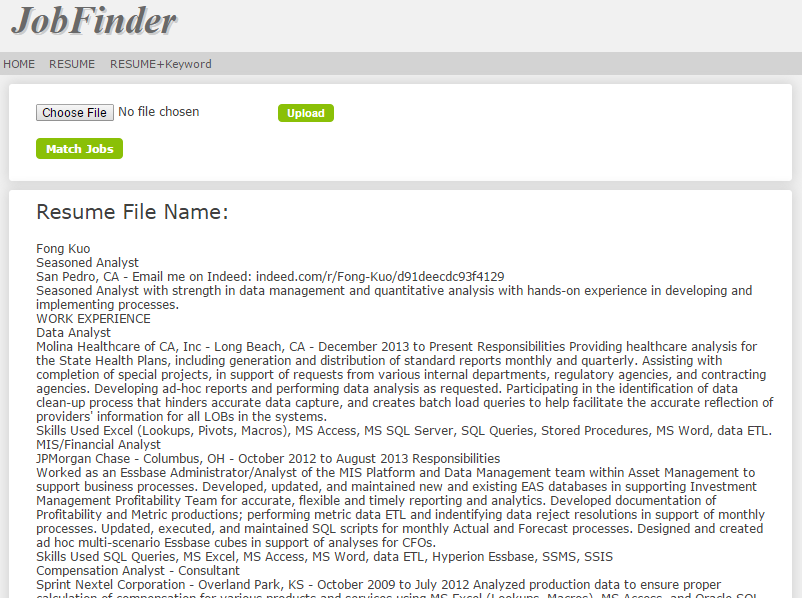
\includegraphics[scale=0.5]{images/upload_resume.png}
  \caption{Upload Resume}
  \label{fig:upload_resume}
\end{figure}

\begin{figure}[htbp]
  \centering
  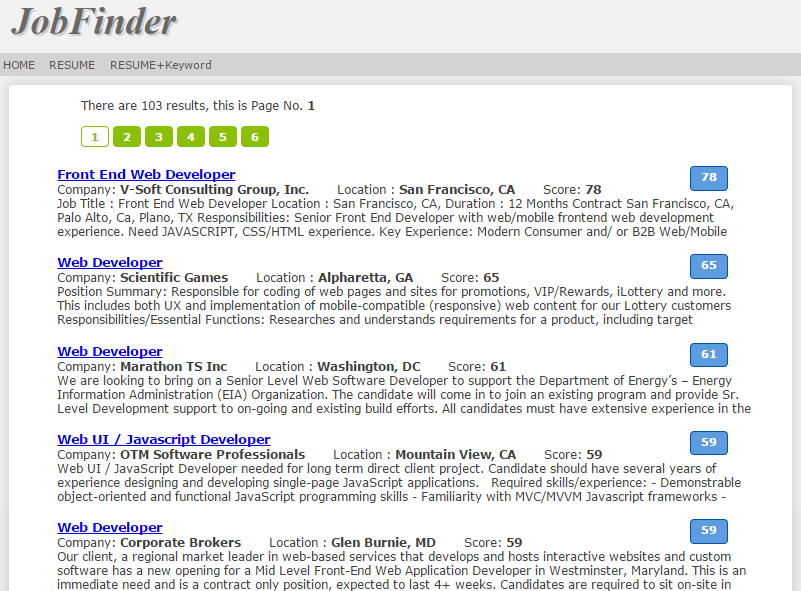
\includegraphics[scale=0.5]{images/match_resume.png}
  \caption{Resume Job matching }
  \label{fig:match_resume}
\end{figure}

\begin{figure}[htbp]
  \centering
  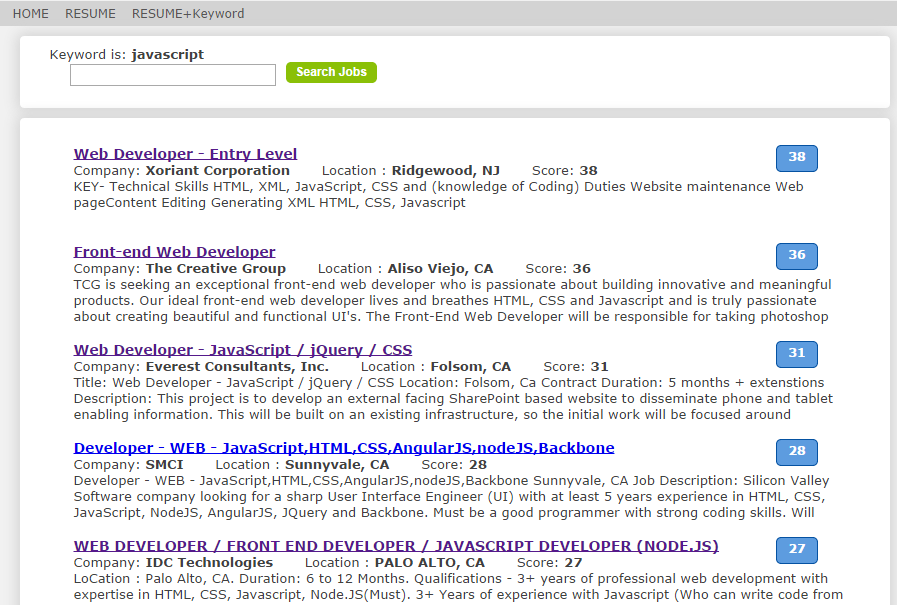
\includegraphics[scale=0.5]{images/keyword_resume.png}
  \caption{Combine the Keyword and Resume Matching}
  \label{fig:keyword_resume}
\end{figure}






